%!TEX root = ./template-skripsi.tex
%-------------------------------------------------------------------------------
%                            BAB III
%               			PEMBAHASAN
%-------------------------------------------------------------------------------

\chapter{DESAIN MODEL}

\section{Tahapan Penelitian}

Diagram \emph{flowchart} dalam gambar \ref{gambar:diagram_experiment} menggambarkan proses modifikasi dari arsitektur \emph{search engine} orisinil menjadi arsitektur \emph{search engine} yang ter-improvisasi.

\begin{figure}[H]
	\centering
	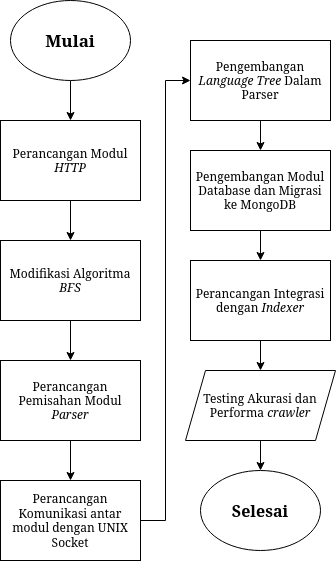
\includegraphics[keepaspectratio, width=7cm]{gambar/experiment-diagram.png}
	\caption{Diagram Tahapan Penelitian}
	\label{gambar:diagram_experiment}
\end{figure}

Proses modifikasi dimulai dengan melakukan konversi modul searah dengan jalannya data ketika proses \emph{crawling}, ini dilakukan untuk mempermudah \emph{testing} terhadap jalannya \emph{crawler}. Modul pertama yang perlu dikonversi adalah modul pengunduhan data atau modul \emph{http}, selanjutnya merancang bagaimana modul \emph{http} dapat berjalan secara \emph{asyncronously} menggunakan \emph{threads}. Modul kedua yang perlu dikonversi adalah \emph{parser}, dalam melakukan konversi \emph{parser} perlu dilakukan pemisahan \emph{parser} dengan modul \emph{http} maka pengkonversian modul \emph{parser} juga dilakukan bersamaan dengan perancangan pemisahan modul tersebut dan metode komunikasi apa yang perlu dilakukan. Modul \emph{database} dikembangkan setelah modul \emph{parser} selesai di-konversikan, karena sumber data-nya berasal dari \emph{parser}, dan selanjutnya juga perlu direncanakan bagaimana \emph{crawler} dapat terintegrasi dengan \emph{indexer}. 

Selain konversi modul, perlu juga dilakukan perancangan algoritma \emph{breadth-first search} yang dimodifikasi untuk meningkatkan akurasi \emph{crawling} per \emph{thread}, algoritma ini akan diintergasikan kedalam modul \emph{http} karena proses \emph{breadth-first search} berkaitan erat dengan proses pengunduhan dan penjelajahan \emph{url}. Hal lain yang perlu diperhatikan adalah ketika proses konversi selesai perlu dilakukan \emph{testing} dan \emph{profiling} untuk memastikan \emph{crawler} termodifikasi ini berjalan lebih cepat daripada \emph{crawler} orisinil.


\section{Modifikasi Arsitektur \emph{Crawler}}

\begin{figure}[H]
	\centering
	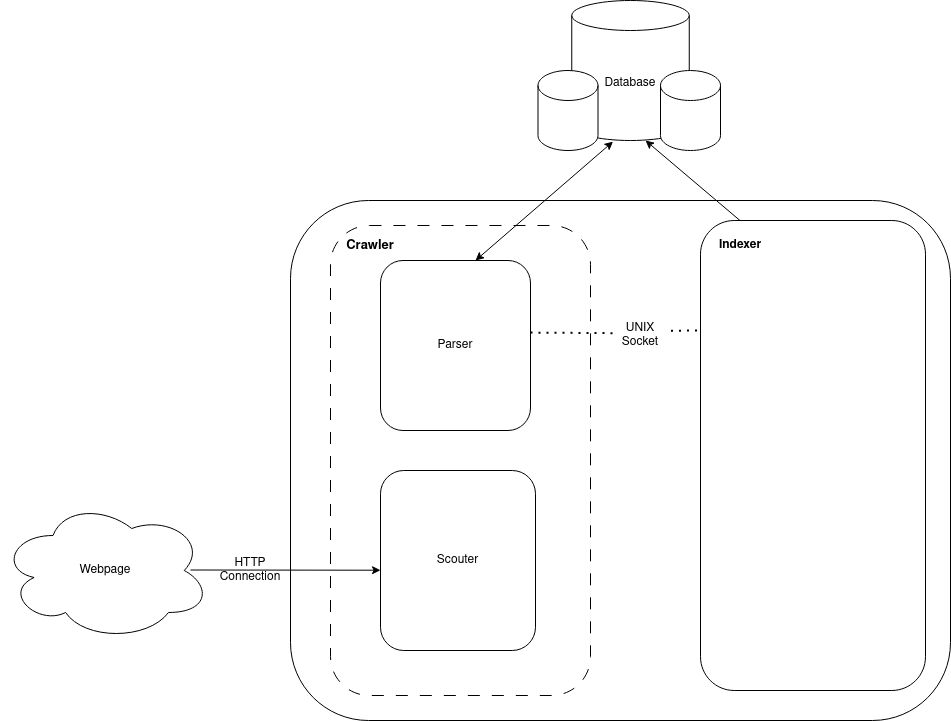
\includegraphics[keepaspectratio, width=15cm]{gambar/crawler-multiprocess-architecture.png}
	\caption{Diagram Arsitektur Crawler Termodifikasi}
	\label{gambar:arsitektur_diagram}
\end{figure}

Dari arsitektur \emph{crawler} yang sudah ada saat ini terdapat beberapa modifikasi yang perlu dilakukan untuk memperbaiki performa proses \emph{crawling}.

\begin{itemize}
  \item Arsitektur ini akan dibagi menjadi 2 \emph{service} yaitu, \emph{crawler} dan \emph{indexer}.
  \item \emph{Service} \emph{Crawler} akan dibagi menjadi dua \emph{process}, \emph{Scouter} dan \emph{Parser}. \emph{Scouter} bertugas sebagai pengunduh halaman \emph{website} dan \emph{parser} bertugas sebagai pembagun \emph{language tree} dan melakukan \emph{input} kedalam \emph{database}.
  \item Jalannya \emph{crawler} dan \emph{indexer} akan secara bersamaan dan otomatis. Untuk mengontrol jalannya \emph{indexer} agar konsistensi data dapat terjaga, 
\end{itemize}

\section{Algoritma modifikasi \emph{Breadth-first search} dengan \emph{domain constraint}}

Untuk menyeragamkan jumlah halaman \emph{web} yang diakses oleh tiap \emph{thread}, algoritma \emph{breadth-frst search} yang digunakan untuk mengunjungi tiap-tiap halaman perlu dimodifikasi. Modifikasi yang dilakukan adalah dengan menugaskan jalannya \emph{crawler} di tiap \emph{thread} sebuah domain \emph{url} tertentu, dan membatasi \emph{url} yang dapat diakses oleh \emph{thread} tersebut sesuai dengan \emph{url} yang telah ditugaskan. Setiap \emph{thread} akan mengambil dan menyimpan \emph{url} di dalam \emph{queue} global, \emph{queue} ini merupakan \emph{multi-lock queue} dengan format yang lebih kompleks dari \emph{queue} normal, ini dilakukan agar tidak terjadi \emph{race condition} antar \emph{thread} ketika mengambil ataupun menyimpan data kedalam \emph{queue} tersebut. Gambar \ref{gambar:diagram_modified_bfs} merupakan ilustrasi dari jalannya algoritma \emph{breadth-first search} termodifikasi.

\begin{figure}[H]
	\centering
	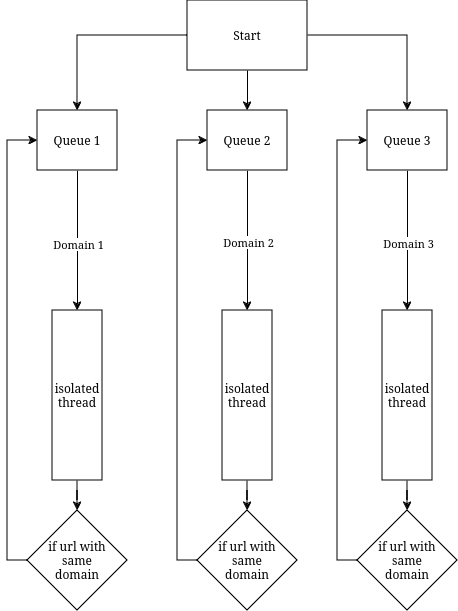
\includegraphics[keepaspectratio, width=8cm]{gambar/modified-bfs-diagram.png}
  \caption{Diagram cara kerja algoritma \emph{breadth-first search} termodifikasi}
	\label{gambar:diagram_modified_bfs}
\end{figure}

\begin{algorithm}[H]
  \caption{Algoritma \emph{breadt first search} termodifikasi}
	\label{Typical_crawling_model}
  \algblockdefx[Name]{ThreadStart}{ThreadEnd}%
    [1][Unknown]{$\textbf{Thread}(#1).Start$}%
    {$\textbf{Thread}.Stop()$}
	\begin{algorithmic}[1]
    \Require{$ P \gets [p_{1}, p_{2}, ..., p_{n}]$ }
    \Function{$BreadthFirstSearch$}{$P$}
      \State $Q \gets {P}$ \Comment{Global multi-lock queue}
      \State $V \gets [..]$ \Comment{visited URLs.} 
      \For{$p_{n} \in Q$}
        \State Async $ScrapPage(p_n)$ \Comment{dijalankan dalam \emph{thread}}
      \EndFor
    \EndFunction
    \Statex
    \Function{$ScrapPage$}{$p_n$}
		    \While{$Q\not=\emptyset$}
		      \State Dequeue $p \in Q$
          \If{$p_{n} (base\_url) = p_{n-1} (base\_url)$}
            \State $ p\_html \gets Fetch(p)$
            \State $Append(V, p)$
            \State $ p\_info \gets ParsePage(p\_html)$
            \For{$links \in p\_info.links$}
              \If{$links \notin V$}
                \State $Append(Q, links)$
              \EndIf
            \EndFor
          \EndIf
		    \EndWhile
    \EndFunction
	\end{algorithmic}
\end{algorithm}

Dalam kode diatas modifikasi dilakukan pada bagian diamana sebelum \emph{links} ditambahkan kedalam \emph{queue}, dilakukan pengecekan terlebih dahulu untuk verifikasi \emph{domain} dari \emph{link} yang akan dimasukkan.

\section{Konversi modul \emph{http}}

Proses pertama yang dilakukan oleh crawler adalah mengunduh halaman \emph{website} atau yang dapat \emph{fetching} , proses ini dilakukan melalui \emph{http get} \emph{request} terhadap \emph{url} dari halaman \emph{website} yang ingin di-unduh. Informasi yang di dapat dari proses \emph{fetching} adalah \emph{url} halaman, konten \emph{html} dari halaman tersebut, dan durasi proses \emph{fetch}. Objek \emph{FetchPage} digunakan untuk menyimpan data-data tersebut.

\begin{figure}[H]
	\centering
	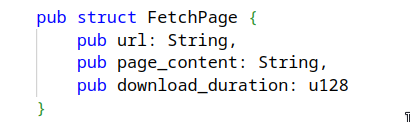
\includegraphics[keepaspectratio, width=10cm]{gambar/http-request-rust-struct.png}
  \caption{Struktur Data yang digunakan untuk operasi \emph{fetching} \emph{http}}
	\label{gambar:http_struct_rust}
\end{figure}

\emph{FetchPage} juga digunakan sebagai \emph{blueprint} dalam definisi modul dan metode \emph{fetching}. Fungsi untuk melakukan \emph{fetching} akan dibuat sebagai \emph{method} dari objek \emph{FetchPage}. \emph{Methdo} \emph{Fetch} merupakan fungsi untuk melakukan pengunduhan, sedangkan \emph{New} adalah fungsi untuk membuat objek \emph{FetchPage} baru yang hanya berisi \emph{url} saja. Untuk mendukung jalannya fungsi \emph{Fetch} secara \emph{asyncronously} dalam modul ini menggunakan dua \emph{library}, yaitu \emph{tokio} dan \emph{reqwest}.

\begin{table}[H]
  \caption{\emph{Library} yang digunakan dalam modul \emph{HTTP}}
  \begin{center}
    \begin{tabular}{ |p{1cm}|p{3cm}|p{7cm}| } \hline
      \textbf{no}.& \textbf{\emph{library}}& \textbf{deskripsi} \\ \hline
      1& \emph{tokio}& Library untuk menjalankan dan mengatur jalannya kode secara bersamaan \\ \hline
      2& \emph{reqwest}& Library untuk membuat dan menjalankan \emph{HTTP} \emph{GET} \emph{request} \\ \hline
    \end{tabular}
  \end{center}
\end{table}

\begin{figure}[H]
	\centering
	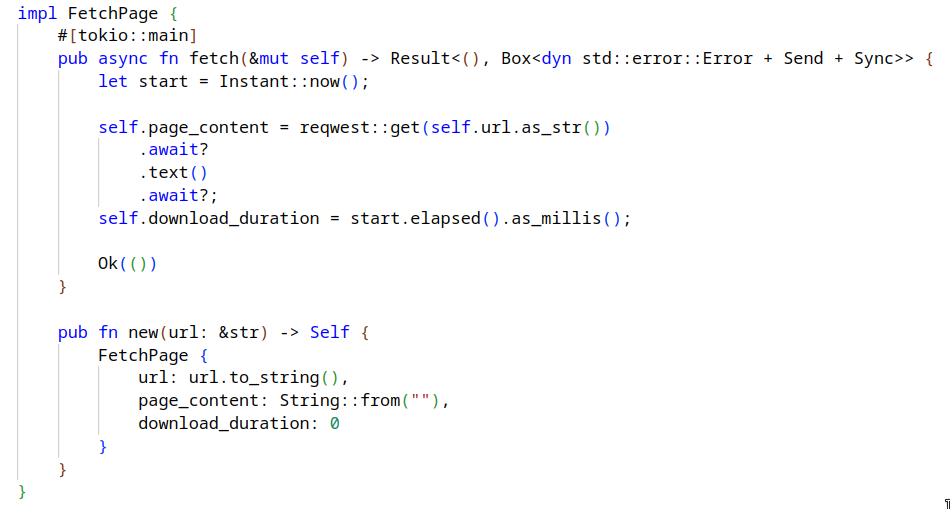
\includegraphics[keepaspectratio, width=15cm]{gambar/http-request-rust-method.png}
  \caption{Fungsi yang digunakan untuk melakuan operasi \emph{fetching} \emph{http}}
	\label{gambar:http_method_rust}
\end{figure}

\section{Perancangan Pemisahan dan Sinkronisasi Proses Module \emph{parser}}

Teks \emph{html} dari modul fetch selanjutnya akan di pindahkan ke modul \emph{parser} untuk diambil informasi-nya. Karena modul \emph{parser} terletak di \emph{process} \emph{rust} yang berbeda, terdapat dua bagian kode yang mengontrol proses ini yaitu,

\begin{enumerate}
  \item Modul sinkronsasi
  \item Modul \emph{parser}
\end{enumerate}

\subsection{Sinkronisasi Menggunakan \emph{UNIX Socket}}

Pengiriman dan sinkronisasi data dalam modul \emph{scouter} dengan dengan modul \emph{parser} dilakukan dengan menggunakan \emph{UNIX Socket}. Sinkronisasi data diatur dengan menggunakan data mentah dari halaman \emph{web} yang sudah diunduh oleh \emph{scouter}, mekanisme dari komunikasi \emph{UNIX Socket} adalah program akan menngirimkan teks \emph{HTML} yang diformat sebagai \emph{memory buffer} yang berbentuk \emph{slice of bytes}.

\begin{figure}[H]
	\centering
	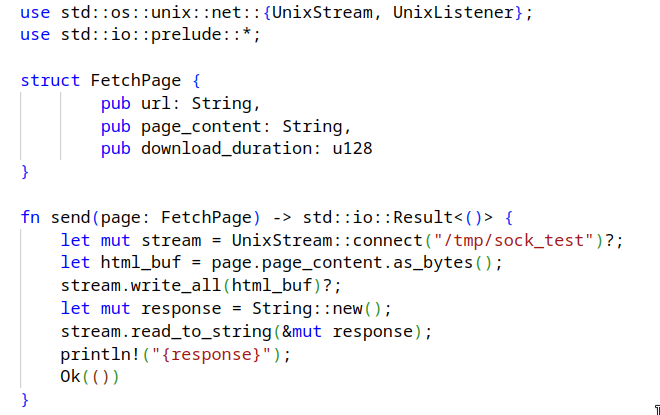
\includegraphics[keepaspectratio, width=10cm]{gambar/unix-sock-send-rs.png}
  \caption{Fungsi yang digunakan untuk melakukan operasi pengiriman teks \emph{html} mengguanak \emph{UNIX Socket}}
	\label{gambar:unix-socket-send}
\end{figure}

\emph{Messages} yang dikirim akan di-konsumsi oleh \emph{receiver} di \emph{process} lain, \emph{messages} ini yang akan di ubah kembali menjadi string dan diproses menuju proses \emph{parsing}. Keseluruhan proses ini perlu menggunakan file sementara dalam sistem \emph{UNIX} sebagai \emph{placeholder} untuk \emph{message}. Proses ini hanya perlu menggunakan \emph{stdlib} dari \emph{rust} untuk menangani pengiriman dan penerimaan \emph{message}.

\begin{figure}[H]
	\centering
	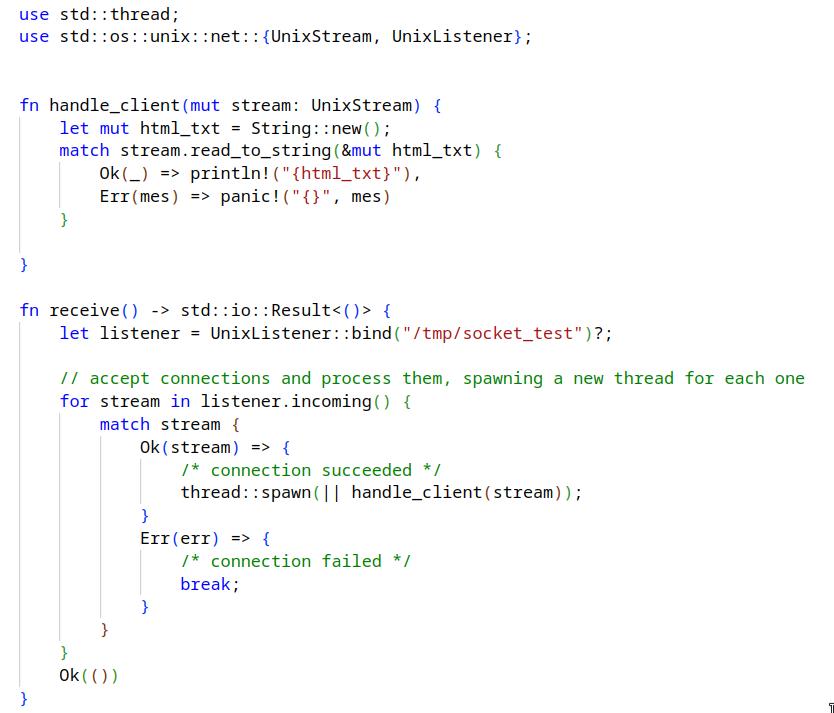
\includegraphics[keepaspectratio, width=12cm]{gambar/unix-sock-receive-rs.png}
  \caption{Fungsi yang digunakan untuk melakukan operasi penerimaan teks \emph{html} mengguanak \emph{UNIX Socket}}
	\label{gambar:unix-socket-receive}
\end{figure}


\subsection{Modul Proses \emph{Parser}}

Data mentah teks \emph{html} yang masuk ke dalam modul \emph{parser} selanjutnya akan di-\emph{parse} untuk mendapatkan informasi-informasi penting dari halaman \emph{web} tersebut. Proses \emph{parsing} ini pada dasarnya hanya membangun struktur \emph{language tree} dari halaman \emph{web} sehingga informasi yang berada di dalam \emph{html tag} lebih mudah untuk di dapatkan. Objek \emph{PageInformation} berfungsi sebagai tempat untuk menyimpan data-data penting per halaman \emph{web}.

\begin{figure}[H]
	\centering
	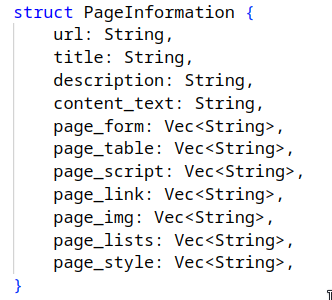
\includegraphics[keepaspectratio, width=7cm]{gambar/parse-object-rs.png}
  \caption{Objek \emph{PageInformation} yang menyimpan data-data hasil proses \emph{parsing} halaman \emph{web}}
	\label{gambar:parse_object}
\end{figure}

Fungsi \emph{parsing} yang akan dipanggil akan dibuat sebagai \emph{method} dari objek \emph{PageInformation}, \emph{parse\_page} sebagai fungsi yang melakukan operasi \emph{parsing} tersebut hanya membangun \emph{language tree} satu kali saat pembuatan variabel \emph{document}. Bagian-bagian \emph{tag HTML} di cari dan di ambil mengguanakn selector yang disesuaikan dengan pola kemunculannya. Informasi tersebut di kumpulkan, beberapa di \emph{input} kedalam bentuk data \emph{vector} dan di masukkan kedalam objek \emph{PageInformation}. Proses ini menggunakan \emph{third-party library} yang bernama \emph{scraper}.

\begin{figure}[H]
	\centering
	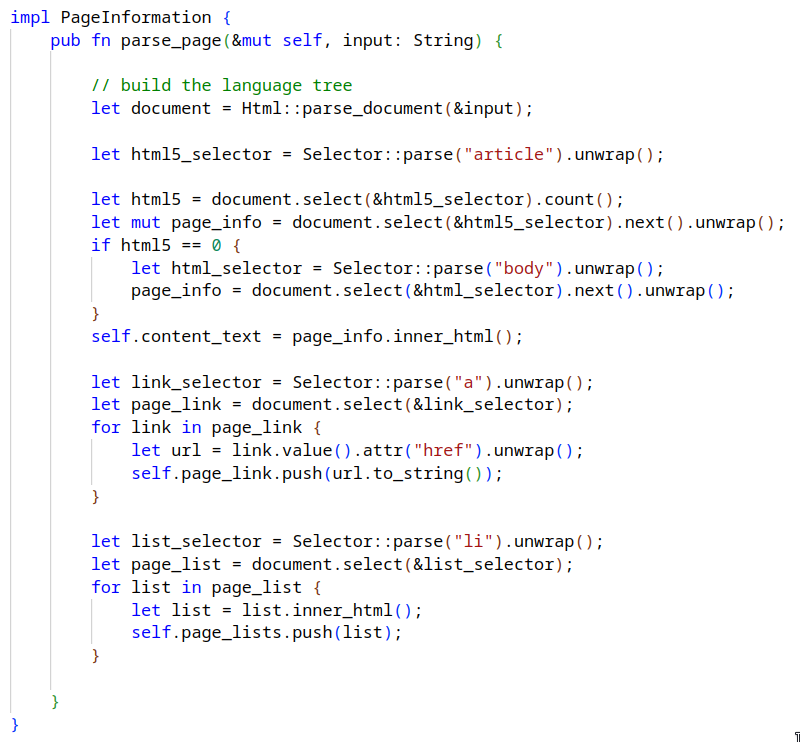
\includegraphics[keepaspectratio, width=15cm]{gambar/parse-method-rs.png}
  \caption{Method \emph{parse\_page} yang mengambil dan menyimpan data-data dari halaman \emph{web} kedalam objek \emph{PageInformation}}
	\label{gambar:parse_method}
\end{figure}

\vspace{0.5cm}

\section{Perancangan konversi modul \emph{database}}

Sebagai cara untuk meningkatkan performa dari \emph{crawler}, penyimpanan data akan diubah dari yang sebelumnya menggunakan \emph{MySql} menjadi menggunakan \emph{MonggoDB}. Struktur dari data yang akan disimpan akan sama tetapi dengan modifikasi terbatas agar dapat tersimpan dengan baik. Pernyimpanan data akan diatur menggunakan Objek untuk mempertahankan konsistensi format data dalam \emph{database}.

\begin{figure}[H]
	\centering
	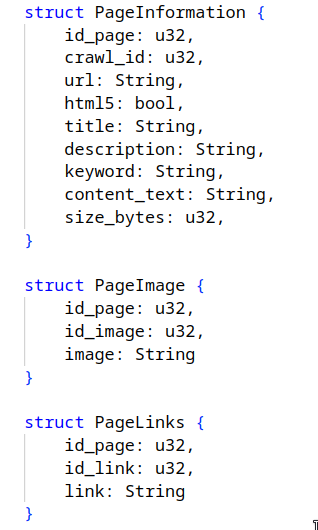
\includegraphics[keepaspectratio, width=5cm]{gambar/rust-db-struct.png}
  \caption{Contoh objek skema penyimpanan data kedalam \emph{database} dalam \emph{rust}}
	\label{gambar:unix_sock_indexer}
\end{figure}

Modifikasi lain yang dapat dilakukan untuk mempercepat proses penyimpanan data adalah dengan menggunakan bulk insert. Berbeda dengan \emph{crawler} sebelumnya yang melakukan penyimpanan pada tiap data satu persatu dengan menggunakan\emph{looping}, \emph{crawler} termodifikasi akan menggunakan mekanisme \emph{bulk insert} yang menjalankan proses penyimpanan hanya sekali.

\section{Perancangan modul sinkronisasi dengan proses \emph{indexing}}

Sinkronisasi dengan proses \emph{indexing} dilakukan dengan memanfaatkan \emph{UNIX Socket}. Sinkronisasi data akan diatur dengan data terformat yang berisi \emph{id\_page} dan \emph{url} dari halaman \emph{web} yang telah disimpan didalam \emph{database}, data ini akan dikirimkan oleh \emph{crawler} setelah menyimpan data dan diterima oleh \emph{indexer}. Dikarenakan \emph{UNIX Socket} merupakan metode komunikasi yang \emph{platform independent} maka tidak perlu ada pengkonversian modul \emph{indexer} kedalam bahasa pemograman \emph{rust}. 

\begin{figure}[H]
	\centering
	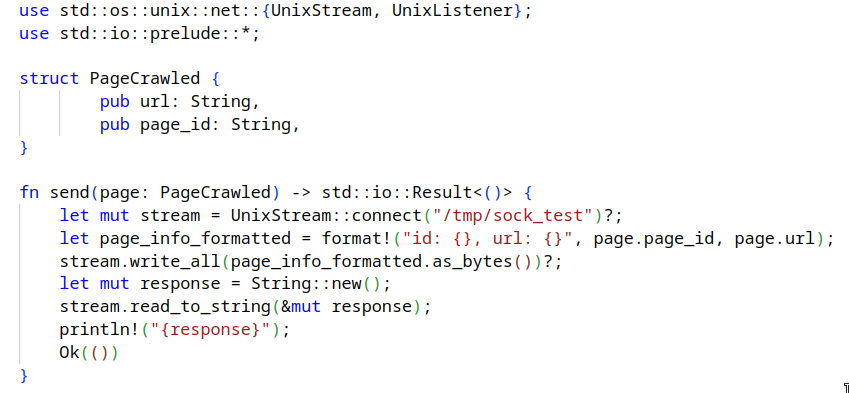
\includegraphics[keepaspectratio, width=15cm]{gambar/unix-sock-indexing.png}
  \caption{Objek dan \emph{method} dalam modul \emph{crawler} sebagai pengirim data menuju \emph{indexer}}
	\label{gambar:unix_sock_indexer}
\end{figure}

\section{Alat dan Bahan Penelitian}

Alat penunjang yang digunakan dalam pengembangan modifikasi \emph{crawler} ini dituliskan dibawah ini:
\begin{itemize}
  \item Laptop dengan konfigurasi Ryzen 4500u 6 core 6 threads, 20GB RAM
  \item Sistem operasi \emph{linux}
  \item \emph{Neovim} sebagai \emph{code editor}
  \item \emph{Docker} untuk mengelola \emph{database} dan \emph{service}
  \item \emph{Rust Programming Language} versi 1.73.0
\end{itemize}

\section{Desain Eksperimen}

\subsection{Modifikasi dan Pengkonversian modul-modul \emph{Crawler}}

Konversi dilakukan sesuai dengan urutan data dalam proses \emph{crawler} orisinil, setiap sub-modul dan proses akan dibuat sebagai modul dengan objek dan \emph{method} untuk memudahkan perpindahan data dari satu sub-modul ke sub-modul yang lain. Konversi dimulai dari sub-modul \emph{http}, sub-modul ini menggunakan \emph{library} \emph{Tokio} dan \emph{reqwest} untuk menjalankan pengunduhan halaman \emph{web}. Data dari sub-modul \emph{http} akan di proses oleh \emph{parser}, sub-modul \emph{parser} dipisah dari sub-modul \emph{http} dalam \emph{process} yang berbeda dan komunikasi antar \emph{process} menggunakan \emph{UNIX Socket}. \emph{Parser} ini digunakan untuk membangun \emph{language tree} dan objeck dalam sub-modul ini berisi data-data yang perlu di ambil dari \emph{html} halaman \emph{web}. Data yang dikumpulkan oleh \emph{parser} akan disimpan dalam database \emph{mongodb}, sebagai \emph{blueprint} dari struktur data dalam \emph{database} tidak akan dirumah untuk menjaga konsistensi data. Setelah data disimpan, modul ini akan mengirim pesan kepada \emph{indexer} untuk memulai proses \emph{indexing}. Gambar \ref{gambar:old_crawler_diagram} merupakan gambaran dari cara kerja \emph{crawler} lama sedangkan gambar \ref{gambar:new_crawler_diagram} merupakan diagram cara kerja \emph{crawler} baru.

\begin{figure}[H]
	\centering
	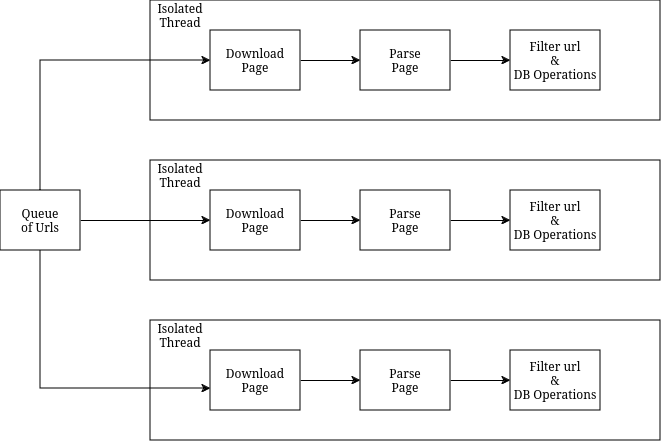
\includegraphics[keepaspectratio, width=10cm]{gambar/old-crawler-multithread-diagram.png}
  \caption{Ilustrasi cara kerja \emph{crawler} lama}
	\label{gambar:old_crawler_diagram}
\end{figure}

\begin{figure}[H]
	\centering
	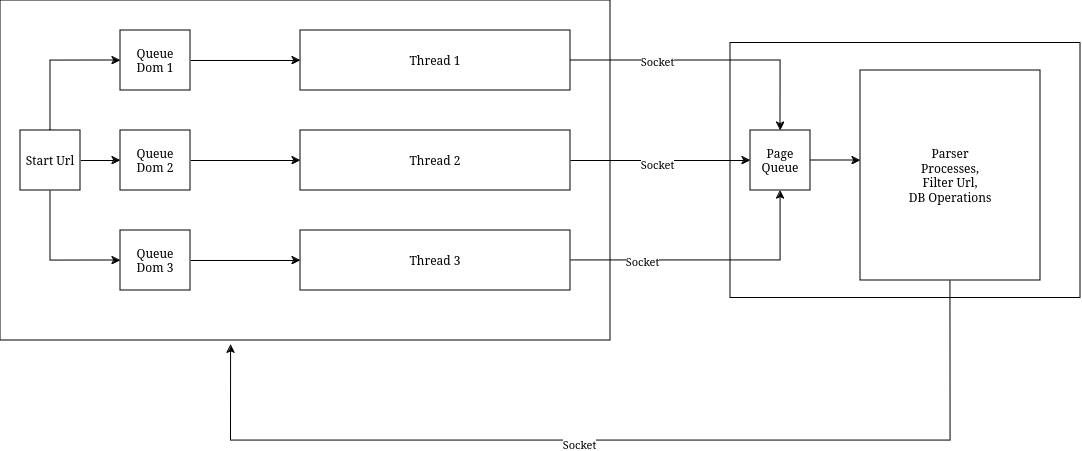
\includegraphics[keepaspectratio, width=10cm]{gambar/new-crawler-multithread-diagram.png}
  \caption{Ilustrasi cara kerja \emph{crawler} baru}
	\label{gambar:new_crawler_diagram}
\end{figure}

\subsection{\emph{Testing}}

Setelah semua modul berhasi di konversikan, perlu dilakukan testing untuk menilai performa \emph{crawler} termodifikas terhadap \emph{crawler} orisinil. Terdapat beberapa poin dari \emph{crawler} yang perlu di-test untuk menilai peningkatan performa yaitu,

\begin{enumerate}
  \item Jumlah halaman yang berhasil dikunjungi selama proses \emph{crawling}
  \item Persentase halaman per-domain yang berhasil dikunjungi relatif terhadap total halaman yang dikunjungi oleh \emph{crawler}
  \item Waktu yang dihabiskan dalam pengambilan informasi dari satu halaman
  \item Konsistensi data yang terkumpul
\end{enumerate}
